\documentclass[]{article}
\usepackage{amsmath}
\usepackage{bm}
\usepackage{graphicx}
\usepackage[hmargin={2.54cm,2.54cm},vmargin={2.54cm,2.54cm}]{geometry}
\usepackage{subfigure}
\usepackage{hyperref}

\graphicspath{{../Images/}}

\title{Advection problem in 3D}

\begin{document}
\maketitle
The code in Tutorials/Amr/Advection\_F is modified to do a 3d case. The Fortran routines contained in the Src\_3d directory from Tutorials/Amr/Advection\_AmrCore/Source is used and routines from\\
Tutorials/Amr/Advection\_AmrCore/Exec/SingleVortex is used. The detailed documentation is given in the AMReX website (https://amrex-codes.github.io/amrex/docs\_html/AmrCore.html), and the changes in 3d are self explanatory.

\section{Run the code}
This example builds the code as a third party by just linking to the amrex library in tmp\_install\_dir/lib. It is done using an automated makefile generation procedure using mkmf (https://github.com/NOAA-GFDL/mkmf) which contains a perl script that creates a makefile taking care of all dependencies (see the git repo for more details). Currently the makefile is already built. If changes are made, then do the following in the Source directory.
\begin{enumerate}
\item ls ../Exec/SingleVortex/*.f90 Src\_3d/*.f90 $>$ path\_names
\item Change the path to tmp\_install\_dir in template.mk (tmp\_install\_dir is located in amrex)
\item ./mkmf/bin/mkmf -t template.mk -p main3d.MPI.gnu.ex path\_names
\item In the source code directory execute -- ./mkmf/bin/mkmf -t template.mk -p main3d.MPI.gnu.ex path\_names -- this will build the makefile
\item make -- will build the executable main3d.gnu.MPI.ex
\item mpirun -np 4 ./main3d.MPI.gnu.ex ../Exec/SingleVortex/inputs
\end{enumerate}
Currently run\_Advection3d.sh has all the commands required to compile and execute the code -- just do sh run\_Advection3d.sh.\\\\
\textbf{Note: The last line in template.mk contains flags from the verbose result of make using AMReX GNUMakefile. There could be more of these flags. These maybe important for optimization.}\\\\
The GNUMakefile is also retained in the SingleVortex directory. To build just do make. Make sure to change the path in Exec/Make.Adv, and also do make clean in the Source directory to remove all .o and .mod files.\\\\
See the visualization section in the AMReX website\\
(https://amrex-codes.github.io/amrex/docs\_html/Chapter11.html) for more details on visualization.\\
Fig.~\ref{fig:Advection3d} shows the result at an instant in time.

\begin{figure}[htpb!]
\centering
\subfigure[]
{
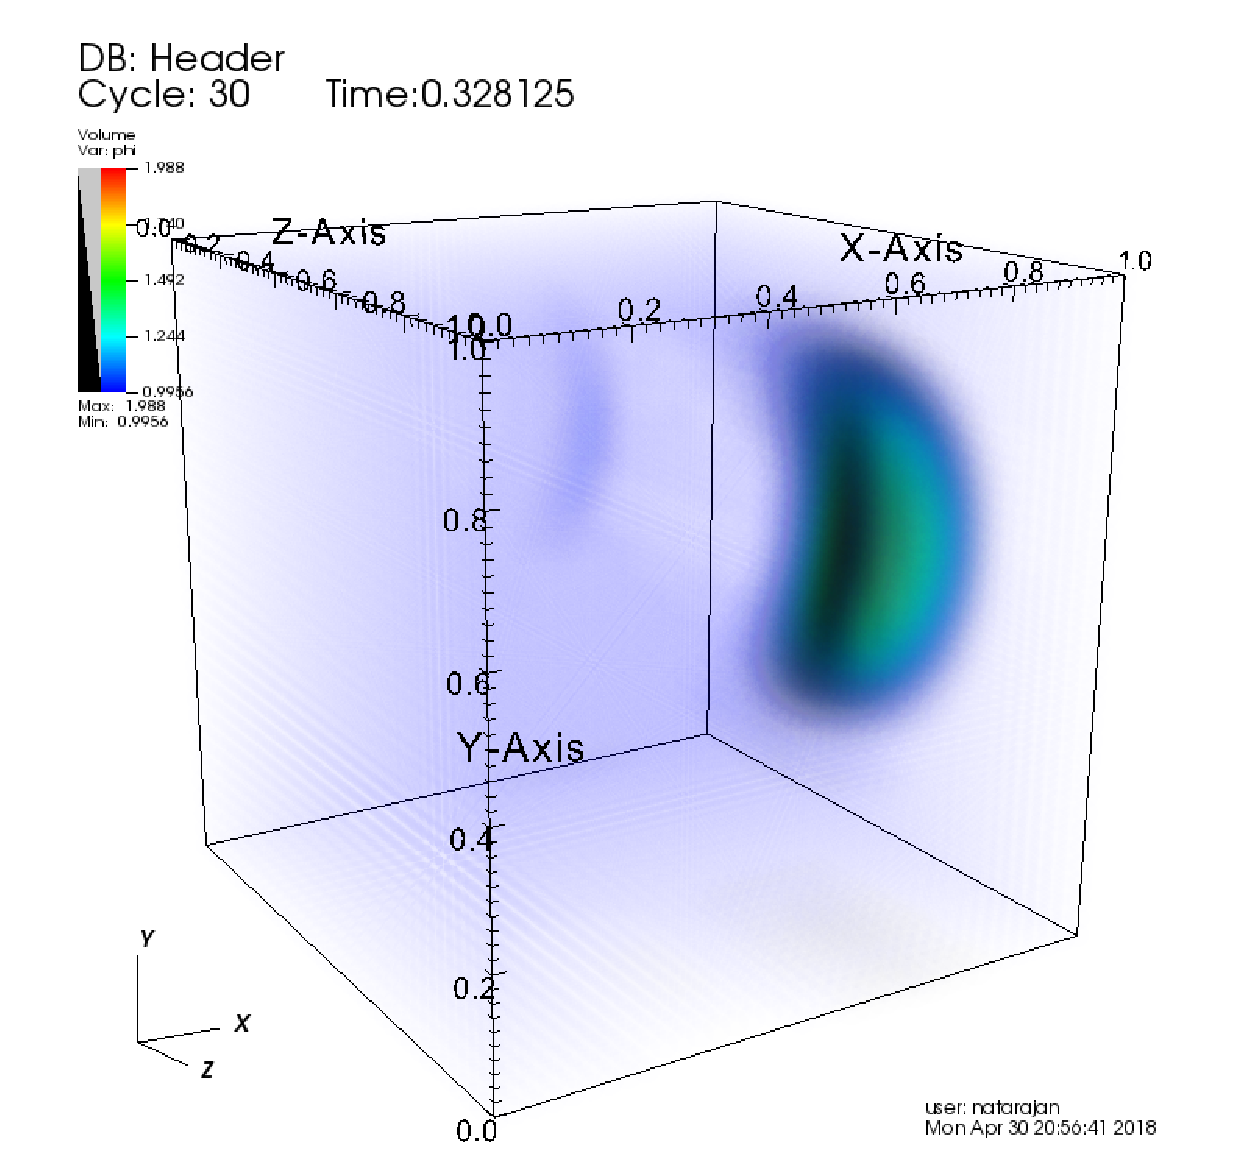
\includegraphics[scale=0.45]{phiInstantaneous}
}\\
\subfigure[]
{
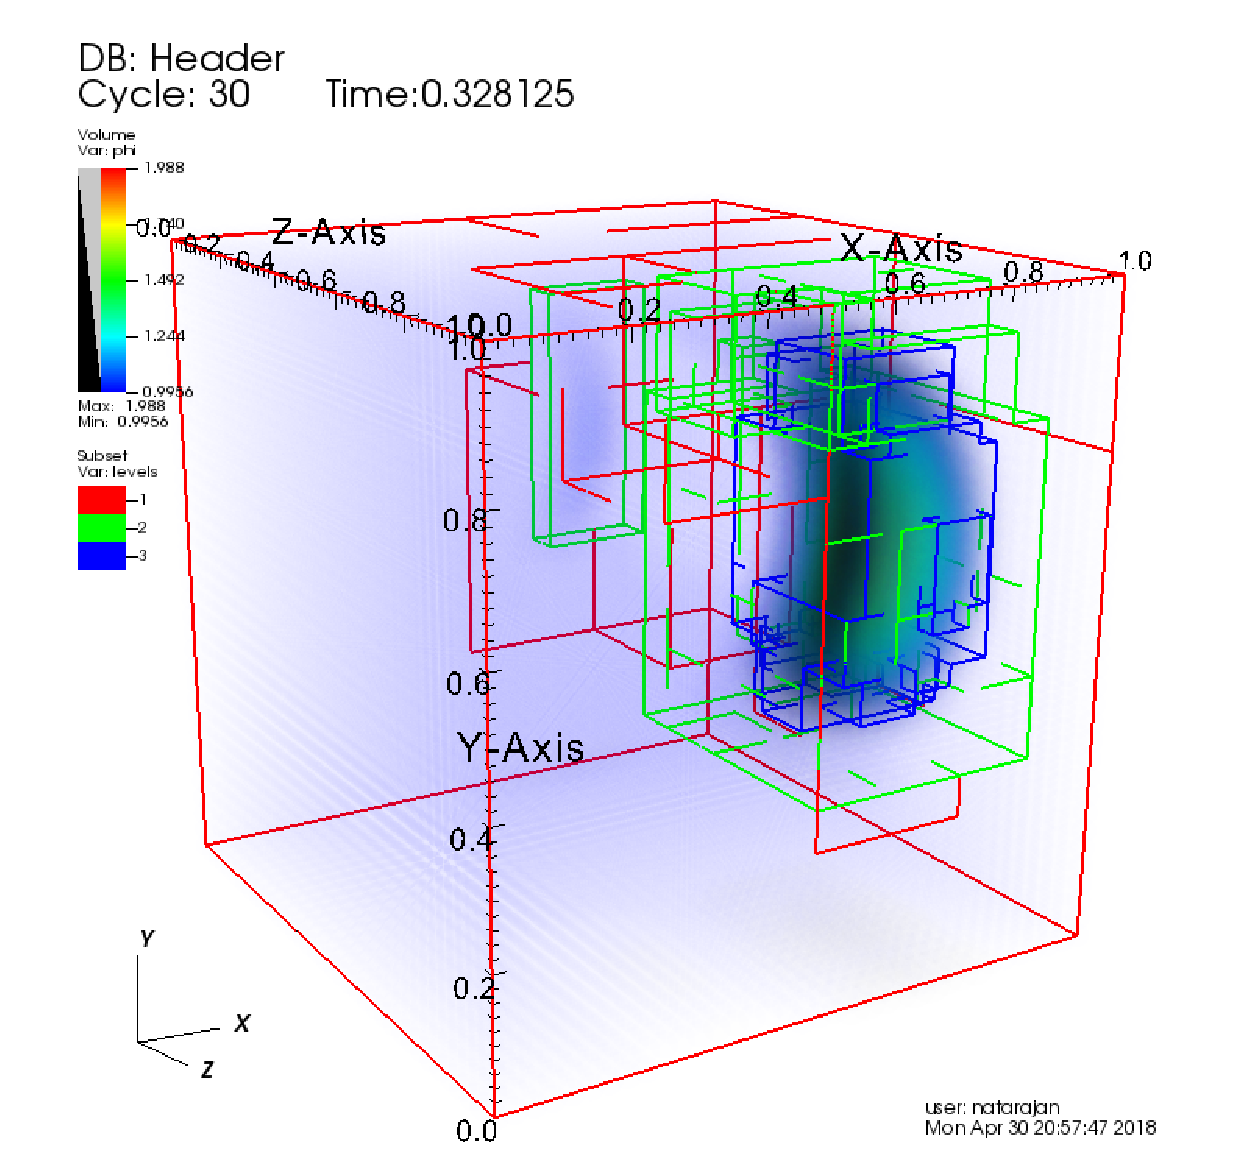
\includegraphics[scale=0.35]{AMRGridLevelsAdvection}
}
\caption{(a) $\phi$ at $t=0.328$ and (b) AMR grid levels.}
\label{fig:Advection3d}
\end{figure}



\end{document}
